\documentclass[../thesis.tex]{subfiles}
 
\begin{document}
 
In this chapter, we propose a model-based local planner for high-speed maneuvering in the off-road navigation application. 
To overcome the highly unpredictable vehicle dynamics in the unstructured terrain, we derive our vehicle model in a data-driven fashion. 
The high-dimensional vehicle model is used as a standpoint of our model-predictive local planner.
 
The local planner is constructed with Rapidly-exploring Random Tree (RRT) \cite{kuffner2000rrt} as its template.
Though sample-based algorithms are generally more suitable for high-dimensional state space planning, it is not straightforward to extend to kinodynamic planning.
To operate the planning process in control space, our planner slightly departs from the standard RRT to perform a certain level of trajectory optimization given the limited computational cycle.
A cost function is designed using traveling time to encourage the vehicle for a more aggressive maneuvering.
 
We use height map algorithm to efficiently process the incoming cloud point data and detect collisions in the future.
The potential obstacles are accumulated on a simplified occupancy grid to produce a collision check grid map.
Finally, the proposed planner is tested on a full-size all-terrain vehicle (ATV) in the off-road environment. 
We show that our planner can perform smooth yet aggressive movements to avoid static obstacles with high speed up to $30 kph$.
 
The chapter is organized as follows:
Section \ref{sec:vehicle_model} summarizes the derivations of two vehicle models. 
In Section \ref{sec:rrt-planner}, we introduce our sample-based planner and detail technical implementations.
Finally, Section \ref{sec:vehicle_model} shows the experimental results and the videos of high-speed navigation.
 
\section{Vehicle Response Model} \label{sec:vehicle_model}
 
\begin{figure}[t]
    	\centering
    	\begin{subfigure}[b]{0.18\linewidth}
    	 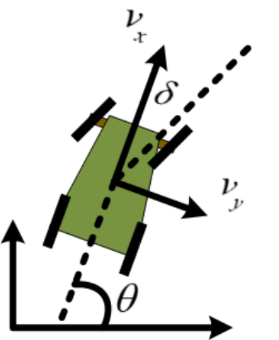
\includegraphics[width=\columnwidth]{./RRTPlanner/fig/vehicle_frame.png}
           	\subcaption{}
           	\label{fig:vehicle_model_frame}
    	\end{subfigure}
    	\begin{subfigure}[b]{0.8\linewidth}
    	 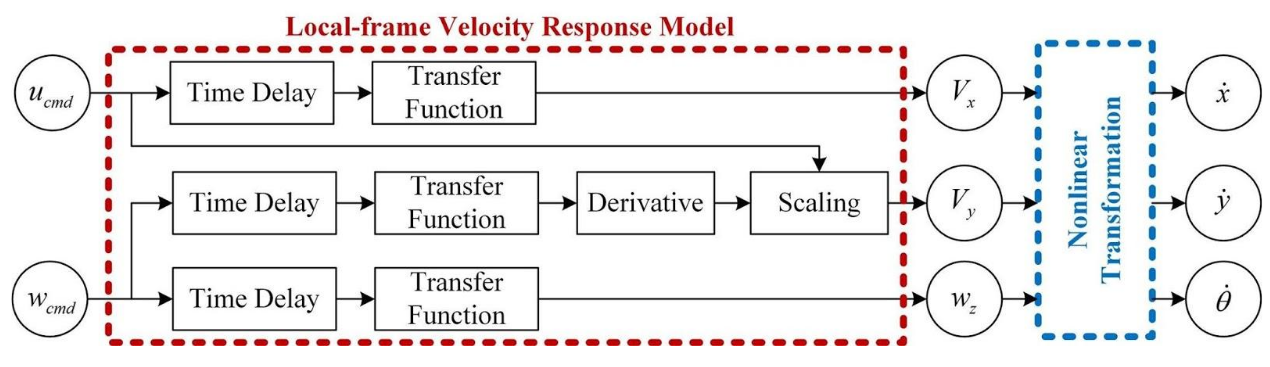
\includegraphics[width=\columnwidth]{./RRTPlanner/fig/vehicle_model_block.png}
           	\subcaption{}
           	\label{fig:vehicle_model_block}
    	\end{subfigure}
    	\begin{subfigure}[b]{0.8\linewidth}
    	 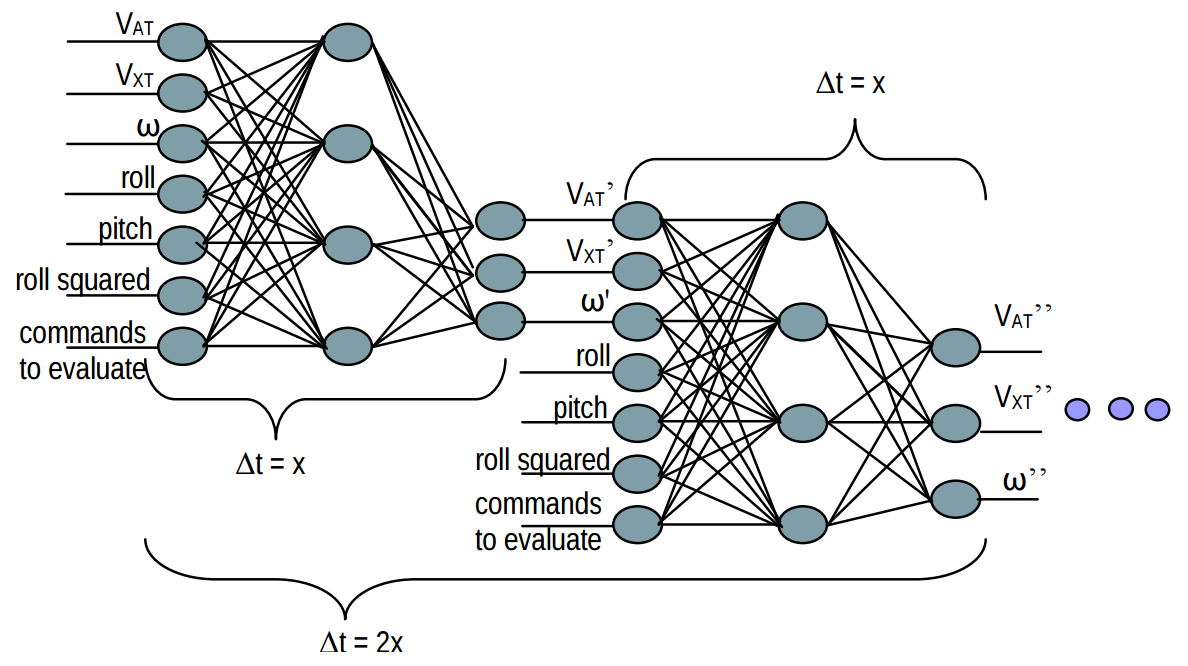
\includegraphics[width=\columnwidth]{./RRTPlanner/fig/neuralnet_model.png}
           	\subcaption{}
           	\label{fig:vehicle_model_net}
    	\end{subfigure}
    	\caption{(a) Notation of vehicle velocity in local frame. (b) Data flow of conventional dynamic response model. The model takes two velocity control commands as input and estimates the velocity response in vehicle frame. (c) Schematic illustration of neural network based response model from \cite{bode2007learning}.}
	\label{fig:vehicle_model}
\end{figure}
 
% Definition/Notation of predictive model
 
The forward predictive model $\dot{x}=f(x,u)$ is defined as a function that maps a pair of control action $u \in \mathcal{A}$ and state $x \in \mathcal{S}$ to the next state. 
As shown in Fig. \ref{fig:vehicle_model_frame}, in our application, the control space consists of the $2DOF$ executed velocity command, \textit{i.e.} forward and rotational velocity, and the state space consists of the actual velocity responses in $2D$ plane, \textit{i.e.} $[v_x, v_y, w]$, in the local frame. 
It is worth mentioning that the sliding velocity $v_y$ is not negligible on the rough terrain, and in fact plays a crucial role in the off-road environment.
 
% Previous works
 
Previous works \cite{kelly2007terrain,howard2006trajectory,howard2005terrain} formulate the predictive models for unmanned ground vehicles (UGV) in a modular fashion, where specialized algorithms are developed for each subsystem and later integrated with some fine tunings. 
Though this approach offers rich semantic representation to allow researchers to better examine the performance of each module, modeling subsystems such as actuator dynamic, vehicle suspension model, and wheel-terrain interaction can be very complex and computationally expensive.
Here, we limit our scope to a more intuitive yet effective method; instead of modularizing the process where the accumulating errors due to the imperfect approximations may propagate and scale up to harm the overall performance, we approximate the predictive model in a more end-to-end fashion.
% The predictive model implicitly includes the effects on
 
% First Model

We derive the model with two different approaches. 
The first approach derives the transfer function based on the standard system identification process. 
The forward and angular velocity responses, \textit{i.e.} $v_x(t)$ and $w_z(t)$, take the forward and angular velocity commands as inputs, respectively. 
The lateral velocity response, on the other hand, uses both commands as input. Our observation is that the UGV experiences lateral sliding whenever the rotational speed changes, with the magnitude of the angular acceleration being proportional to the forward velocity. 
The corresponding block diagram is summarized in Fig. \ref{fig:vehicle_model_block}. 
The relative position with respect to the origin in local frame can be calculated by integrating through velocity space.
 
% Second model
For the second approach, we implement the neural network model based on previous work \cite{bode2007learning}. As shown in Fig. \ref{fig:vehicle_model_net}, the neural network takes additional information, such as roll, pitch, and yaw angle, as its input. Note that the squared roll angle is also provided because, from a dynamics standpoint, the vehicle should respond in a near symmetrical manner if it is rolled to the right or rolled to the left.
We refer two models as \textit{Conventional Dynamic Model} and \textit{NNet Model} for convenience in the later section.
% We verified the performances of the two models on predicting vehicle states response on the full-size all-terrain vehicle in Section \ref{sec:rrt-experiments}. The two models are referred as 
 
 
\section{Planner Design} \label{sec:rrt-planner}
 
 
\begin{figure}[t]
    	\begin{center}
    	 \centerline{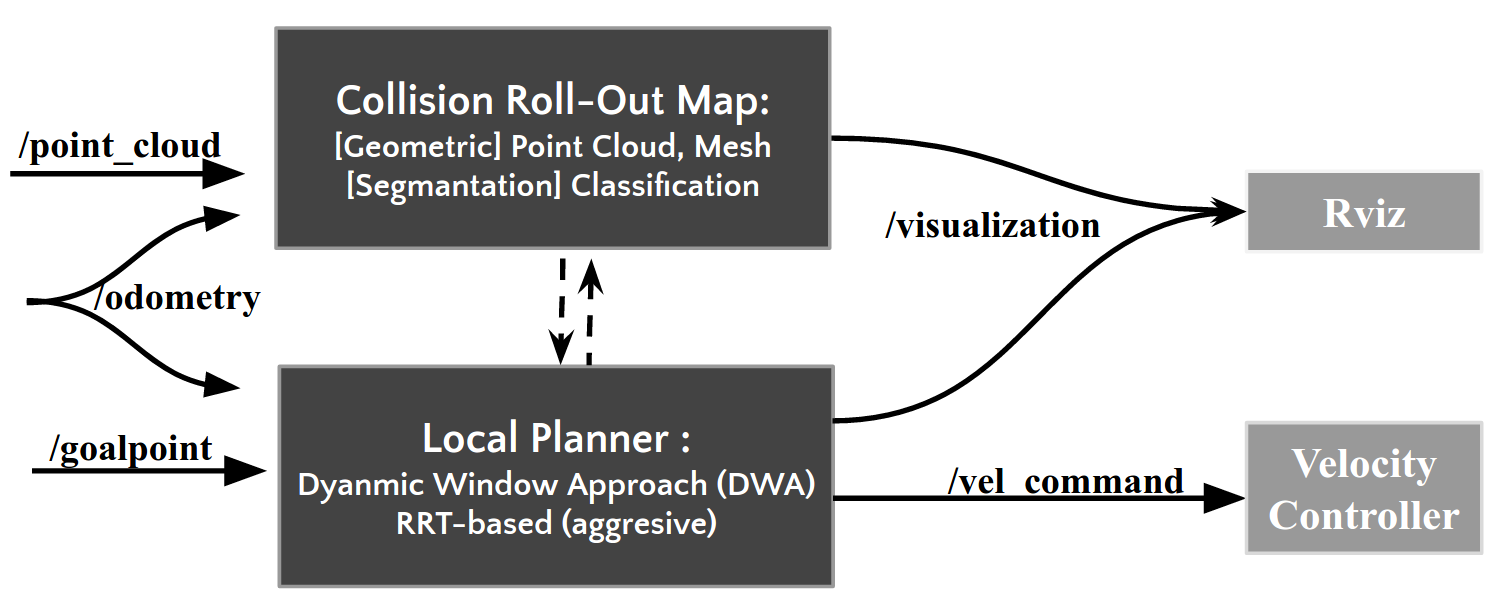
\includegraphics[width=0.8\columnwidth]{./RRTPlanner/fig/planner_module.png}}
           	\caption{Block Diagram of our planner API.}
           	\label{fig:planner_module}
    	\end{center}
\end{figure}
 
The block diagram of our planner is shown in Fig. \ref{fig:planner_module}. 
It can be separated into two modules with respect to functionality. 
The collision check module constructs a global simplified occupancy grid given the point cloud data and the odometry. 
The local planner module takes the odometry and the goal state as inputs, performs minimal calculations, and finally sends the velocity commands directly to the onboard velocity controller.
The two modules interact with each other in the way that the local planner acquires collision detections from the roll-out map.
% then communicated with the RRT-based planner for collision check service.
The detail of two modules is described as follows:
 
 
\subsection{Collision Check Module}
 
Occupancy grid is a commonly-used data structure for obstacles detection. 
It stores one or multiple probabilities in each grid cell and increases or decreases them based on sensor model. 
Since our testing scenario is relatively flat without noise, a simplified version of occupancy grid is used in the matter of fast implementation, in which we replace the probabilities with a counter. 
Three different methods for obstacles segmentation are investigated and described below:
 
\begin{figure}[t]
    	\centering
    	\begin{subfigure}[b]{0.3\linewidth}
    	 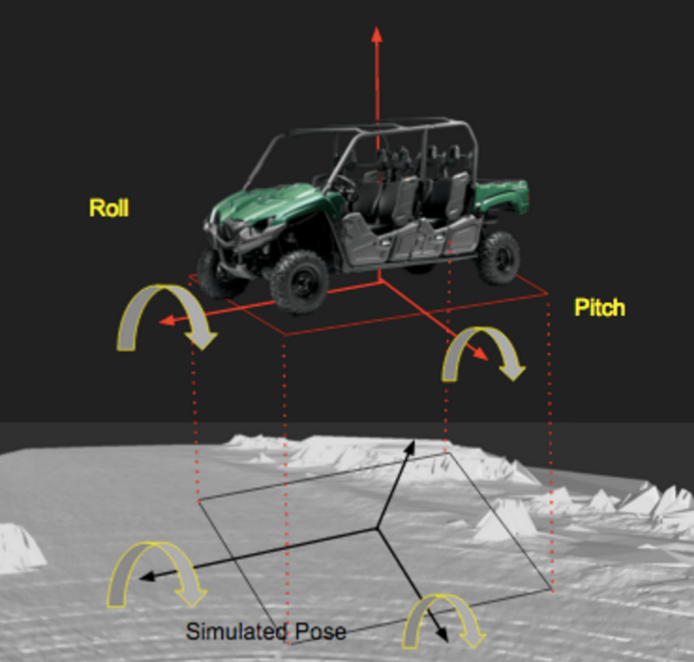
\includegraphics[width=\columnwidth]{./RRTPlanner/fig/mesh.png}
           	\subcaption{Mesh with ODE simulation}
           	\label{fig:collision_mesh}
    	\end{subfigure}
    	\begin{subfigure}[b]{0.3\linewidth}
    	 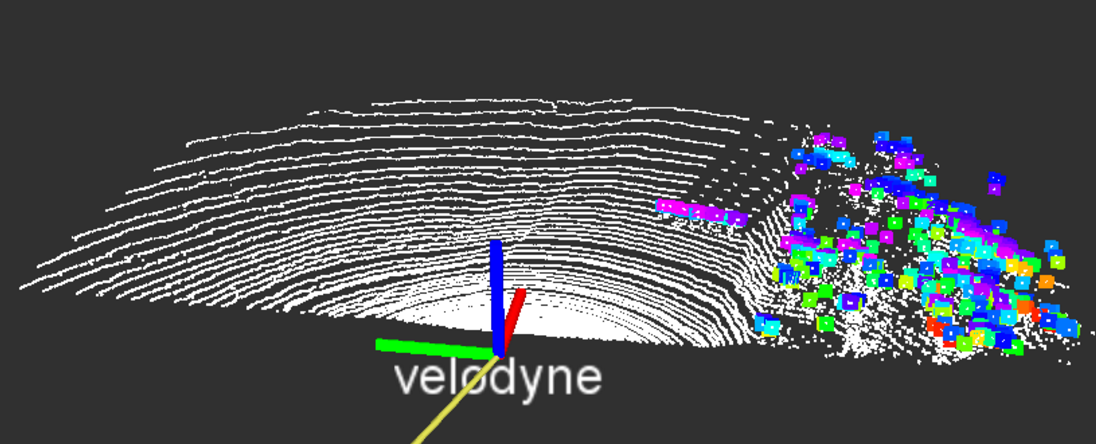
\includegraphics[width=\columnwidth]{./RRTPlanner/fig/ransac.png}
           	\subcaption{RANSAC segmentation.}
           	\label{fig:collision_ransac}
    	\end{subfigure}
    	\begin{subfigure}[b]{0.3\linewidth}
    	 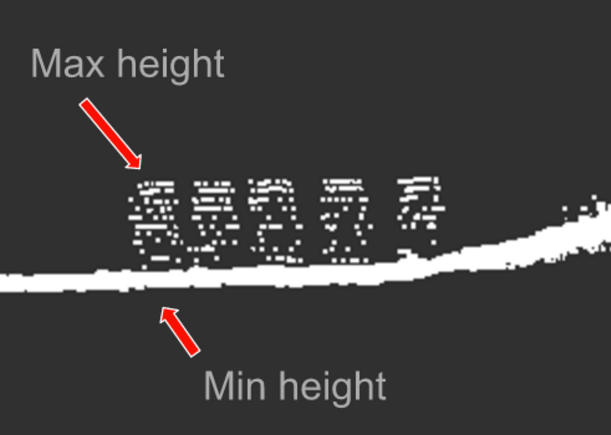
\includegraphics[width=\columnwidth]{./RRTPlanner/fig/height_map.png}
           	\subcaption{Height map algorithm}
           	\label{fig:collision_height_map}
    	\end{subfigure}
    	\caption{Three different methods of collision check. Note that for (b), the original and the processed point cloud is represented by white and colored dot, respectively.}
	\label{fig:collision}
\end{figure}
 
 
\subsubsection{i. Mesh Representation with Simulation in Open Dynamic Engine (ODE) \cite{wettergreen2012developing}}
The original method implemented on the vehicle uses ODE and mesh data to simulate the vehicle pose on the ground. 
The collision is reported if 1) an intersection is detected between the vehicle and the mesh map or 2) the simulated roll or pitch angle is beyond the user-defined thresholds.
 
\subsubsection{ii. Plane Removal with RANSAC Segmentation \cite{fischler1981random}}
The second approach for collision check module is using RANSAC segmentation from Point Cloud Library (PCL) to fit the plane model. 
In our case, the plane model is the ground of our testing environment. 
We extract the outliers from RANSAC for obstacle detection. 
As shown in Fig. \ref{fig:collision_ransac}, the white point cloud is the original data, while the colored point cloud is the outliers from RANSAC.
 
\subsubsection{iii. Height Map Algorithm}
The third method we used is height map algorithm, which is a simple yet efficient algorithm regarding computation. 
It calculates the height differences within one grid. If the height difference is greater than a user-defined threshold, the obstacle is categorized as an obstacle. 
As shown in Fig. \ref{fig:collision_height_map}, since the artificial obstacle is approximately $1.5$ meters, we set the threshold to be $1$ meter. 
% Thus, it will be recognized as an obstacle.
 
 
% conclusion
Since collision check is the most computationally expensive part of our system and we cannot afford to collide our platform with the obstacles, efficiency and reliability are the most important requirements. 
Though the mesh representation is a good approach for future application, it is not feasible in our scenario regarding computation consumption. 
The RANSAC segmentation, on the other hand, is sensitive to off-road conditions; the plane model cannot be perfectly fit on rough terrain. 
In addition, the dusty environment in off-road driving creates noises and interferences to the Lidar. 
Considering our requirements and the discussion mentioned above, we choose height map algorithm as our final approach. 
It is the fastest and the most reliable. 
Furthermore, to optimize the computing efficiency, we use bitwise operation instead of multiplication and dilate the obstacle size to increase the robustness of our system.
 
\subsection{Sample-based Planner Module}
 
% Intro
Instead of using traditional search-based planners such as \textbf{A*} or \textbf{D*}, we use a sample-based planner as our development platform. 
This critical choice comes from an insight that sample-based planner is more efficient for solving a high-dimensional planning problem, which gives us a powerful tool when we want to utilize a more complex dynamic vehicle model for state propagation.
% In addition, maneuvering in the wilderness can be seen as a generalized planning problem where discretizing the world based on resolution might not generate a smooth path.
 
\subsubsection{Simulation}
 
\begin{figure}[t]
    	\centering
    	\begin{subfigure}[b]{0.3\linewidth}
    	 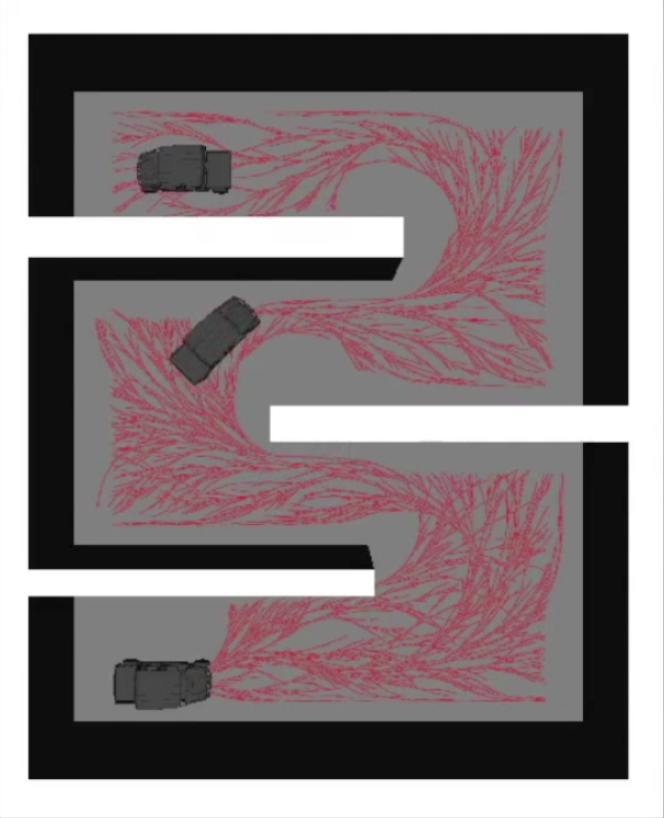
\includegraphics[width=\columnwidth]{./RRTPlanner/fig/rrt-sim-maze1.png}
           	\subcaption{}
           	\label{fig:rrt-sim-maze1}
    	\end{subfigure}
    	\begin{subfigure}[b]{0.3\linewidth}
    	 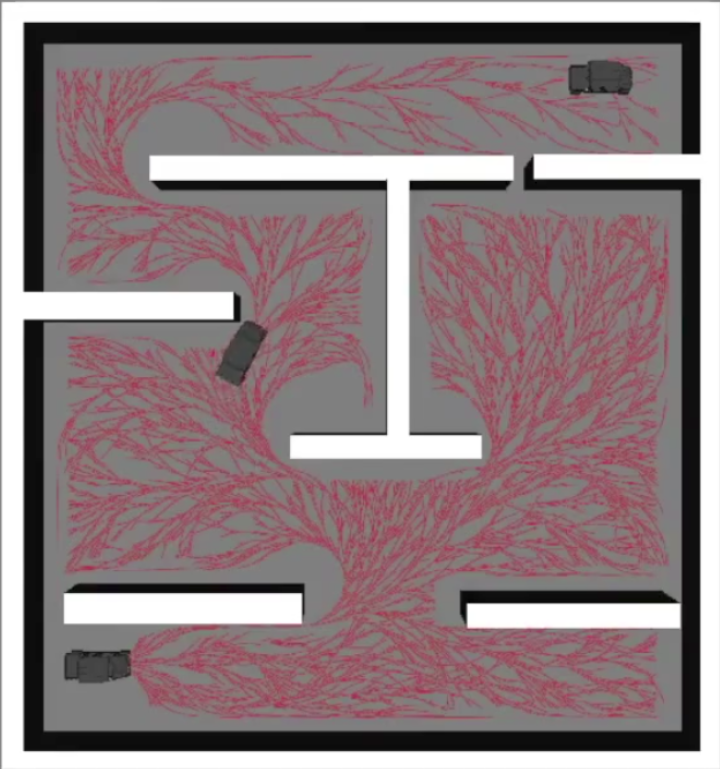
\includegraphics[width=\columnwidth]{./RRTPlanner/fig/rrt-sim-maze2.png}
           	\subcaption{}
           	\label{fig:rrt-sim-maze2}
    	\end{subfigure}
    	\caption{Simulation of RRT planner with vehicle model derived in Sec. \ref{sec:vehicle_model}}
	\label{fig:rrt-sim-maze}
\end{figure}
 
 
\begin{table}[t]
    	\centering
    	\caption{Simulation Benchmark}
    	\label{table:simulation-benchmark}
    	\begin{small}
    	\begin{sc}
    	\begin{tabular}{ccccc}
           	\toprule
                   	& PDST \cite{ladd2005motion} & EST \cite{hsu1997path} & RRT \cite{kuffner2000rrt} & KPIECE \cite{csucan2009kinodynamic} \\
           	\midrule \midrule
           	time & 15.04 & 15.05 & \textbf{15.03} & 15.07 \\
           	solution clearance & 1.63 & 1.54 & \textbf{1.38} & 1.70 \\
           	solution difference & 1.05 & 1.11 & \textbf{0.98} & 1.30 \\
           	\toprule
    	\end{tabular}
    	\end{sc}
    	\end{small}
\end{table}
 
% Simulation
Our planner is built upon Open Motion Planning Library (OMPL) \cite{sucan2012the-open-motion-planning-library}, an open-source motion planning library that includes a broad range of sample-based planners and a built-in simulation platform called \textit{OMPL.app}.
The template of the sampled-based planner is determined from simulations where we generate mazes scenarios and implement the vehicle response model on several available off-the-shelf planners. 
Table \ref{table:simulation-benchmark} summarizes the simulated benchmark result, while Fig. \ref{fig:rrt-sim-maze} shows the simulation environments. 
The demo video available at \url{http://ppt.cc/sBLAh}. 
We observe that the RRT algorithm gives a faster solving time and a smaller path clearance under our vehicle model constraints.
With other advantages such as flexibility and extendibility, we use RRT as our planner template and extend it for our purpose.
 
 
\subsubsection{Implementation Details}
 
\begin{figure}[t]
    	\begin{center}
    	 \centerline{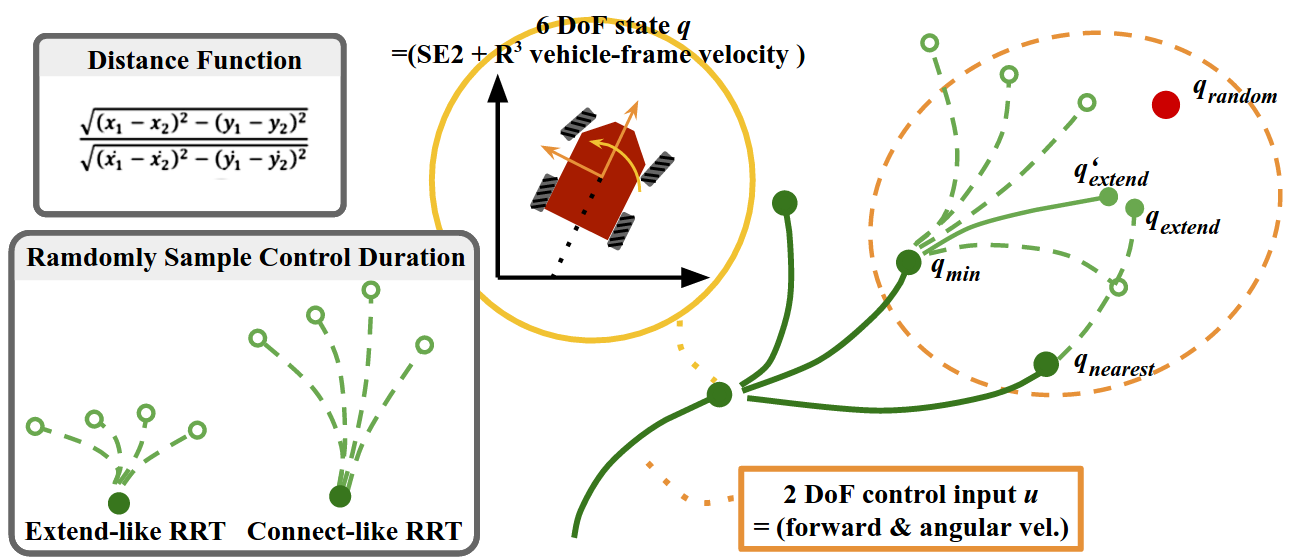
\includegraphics[width=0.8\columnwidth]{./RRTPlanner/fig/rrt.png}}
           	\caption{The visualization of RRT-based planner.}
           	\label{fig:rrt}
    	\end{center}
\end{figure}
 
% RRT visualize
Fig \ref{fig:rrt} visualizes the RRT tree. 
Each node represents a $6$ DoF state, $q=[x,y, \theta ,v_{forward}, v_{sliding}, w]^T$. 
The first three terms represent the state in standard SE2 space, and the last three terms stand as the velocity in vehicle frame on a 2D plane. 
For control space, we follow the convention used in Section \ref{sec:vehicle_model}, which includes $2DOF$ forward and angular velocity.
 
% shooting method and control consistency
After a random state $q_{random}$ is sampled, RRT extends its leaf by determining a sequence of control input and its operation duration toward an extended state $q_{extend}$.
To perform a smooth control throughout the trajectory for off-road navigation, we first uniformly sample the forward velocity command within an adjustable region.
This command region is determined at run-time based on the previously issued commands, current vehicle status, and previously executed path so that the vehicle will hold the velocity consistency without jerky output.
Then, the shooting method is used to determine the angular velocity command.
 
% random step size
As shown in the dotted circle in Fig. \ref{fig:rrt}, the basic RRT-like algorithm preserves a fixed extended step size throughout planning time.
While using a larger step size may decrease solving time yet result in a jerky trajectory, the trajectory propagated with a smaller step size is usually smoother but computationally expensive.
The former one is usually referred to \textit{Connected RRT}, and the latter one is called \textit{Extended RRT}.
In our implementation, instead of fixing the control duration as a hyper-parameter, we randomly sample the control duration.
Our motivations come from the results of our maze simulations, where we observe that tuning the control duration greatly affects the planner performance in different maze configuration.
We believe loosening the step size constraint with such random sample mechanism will generalize our planner for various situations encountered in off-road environments.
 
% optimization
Optimal kinodynamic motion planning for a sample-based planner can be very computationally expensive.
As described in Section \ref{sec:sample_based_planning}, moving from RRT toward RRT* includes two more optimization steps in each iteration: (1) reconnecting to an extended state, and (2) tree edges trimming.
% Finding an optimal plan is crucial for motion planning but computationally expensive if using a sample -based control-space planner.
Here, we implement a time-optimal RRT* algorithm motivated from \citet{hwan2011anytime}.
However, only the first of two optimization steps is applied because the trimming process includes updating the whole children tree, which will trade off with planning time.
The extend function in the first procedure is implemented slightly different from the basic version in that instead of connecting $q_{extend}$ directly to $q_{min}$, we apply shooting method and replace $q_{extend}$ with $q^{''}_{extend}$.
The intuition is that it is nearly impossible to propagate to the \textit{same} node in 6 DoF state space with arbitrary control commands.
The replacement of $q_{extend}$ is accepted only if the new state $q^{''}_{extend}$ is close enough to $q_{extend}$.
Finally, we also follow the same setting by using the traveling time instead of standard Euclidean distance as the cost function.
The planner thus optimizes the trajectory by minimizing the traveling time and is encouraged to maneuver agilely under the dynamics constraints.
 
% re-planning
The re-planning process is designed as follows: at the beginning of each planner loop, the vehicle status, collision check map, and goal state are updated to formulate an RRT control-space planning problem.
The problem is solved multiple times, and the best solution in each iteration is stored.
When the computational time exceeds, the solution with minimal cost is outputted for execution.
Note that the growth tree is abandoned when the next solving iteration starts.
In practice, such design helps prevent the planner from publishing poor solution if bad tree structure is built at the beginning of growth stage.
We admit that if an optimal solution can be obtained from one single shot, the re-planning setting would have changed significantly \cite{ferguson2006replanning}.
It is also worth mentioning that there is a time delay between the time when the vehicle status is updated and the time when the velocity command generated by RRT-based planner is executed.
To effectively capture the latency, the starting vehicle state, \textit{i.e.} the root of RRT, is simulated by propagating the current vehicle with the delayed time using the vehicle model derived in the previous section.
The parameters used in our local planner are listed in Table \ref{table:rrt-parameters}.
 
\begin{table}[t]
    	\centering
    	\caption{Planner Hyper-parameter}
    	\label{table:rrt-parameters}
    	\begin{small}
    	\begin{sc}
    	\begin{tabular}{ccc}
           	\midrule \midrule
           	\multicolumn{2}{c}{Goal Bias} & 0.7 \\
           	\multicolumn{2}{c}{Planner Rate} & 2 Hz \\
           	\multicolumn{2}{c}{Solving Rate} & 20 Hz \\
           	\multicolumn{2}{c}{Control Duration} & 1.5--6 sec \\
           	\multirow{2}{*}{Control Input} & Forward & 10--30 kph \\
           	                                                       	& Angular & -0.5--0.5 rad/s \\
           	\toprule
    	\end{tabular}
    	\end{sc}
    	\end{small}
\end{table}
 
 
\section{Experiments and Analysis} \label{sec:rrt-experiments}
 
 
\begin{figure}[t]
    	\begin{center}
    	 \centerline{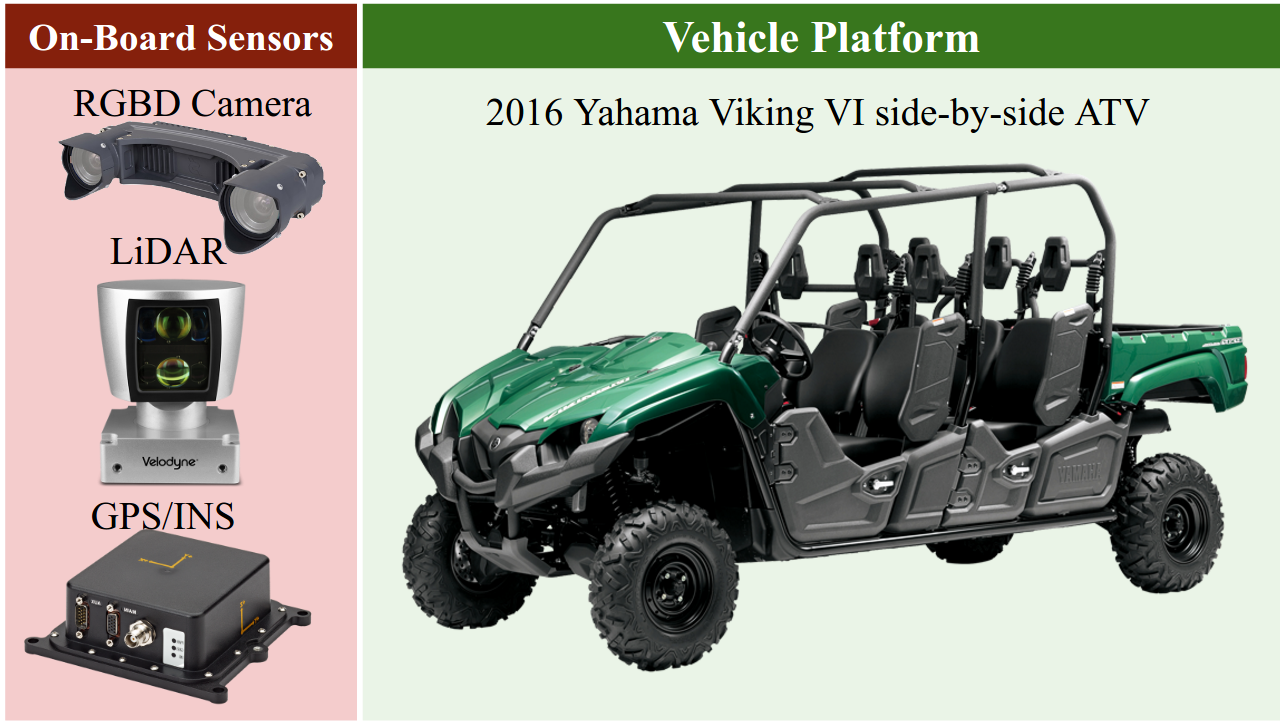
\includegraphics[width=0.7\columnwidth]{./RRTPlanner/fig/viking.png}}
           	\caption{The testing vehicle platform and the onboard sensor.}
           	\label{fig:viking}
    	\end{center}
\end{figure}
 
We use Yamaha Viking VI side-by-side ATV as our main testing platform. 
As shown in Fig. \ref{fig:viking}, the vehicle is equipped with the custom drive-by-wire system, velocity controller, and navigation sensors such as GPS/INS, LiDAR, and RGB-D camera.
 
 
\subsection{Vehicle Model Verification}
 
\begin{figure}[t]
    	\begin{center}
    	 \centerline{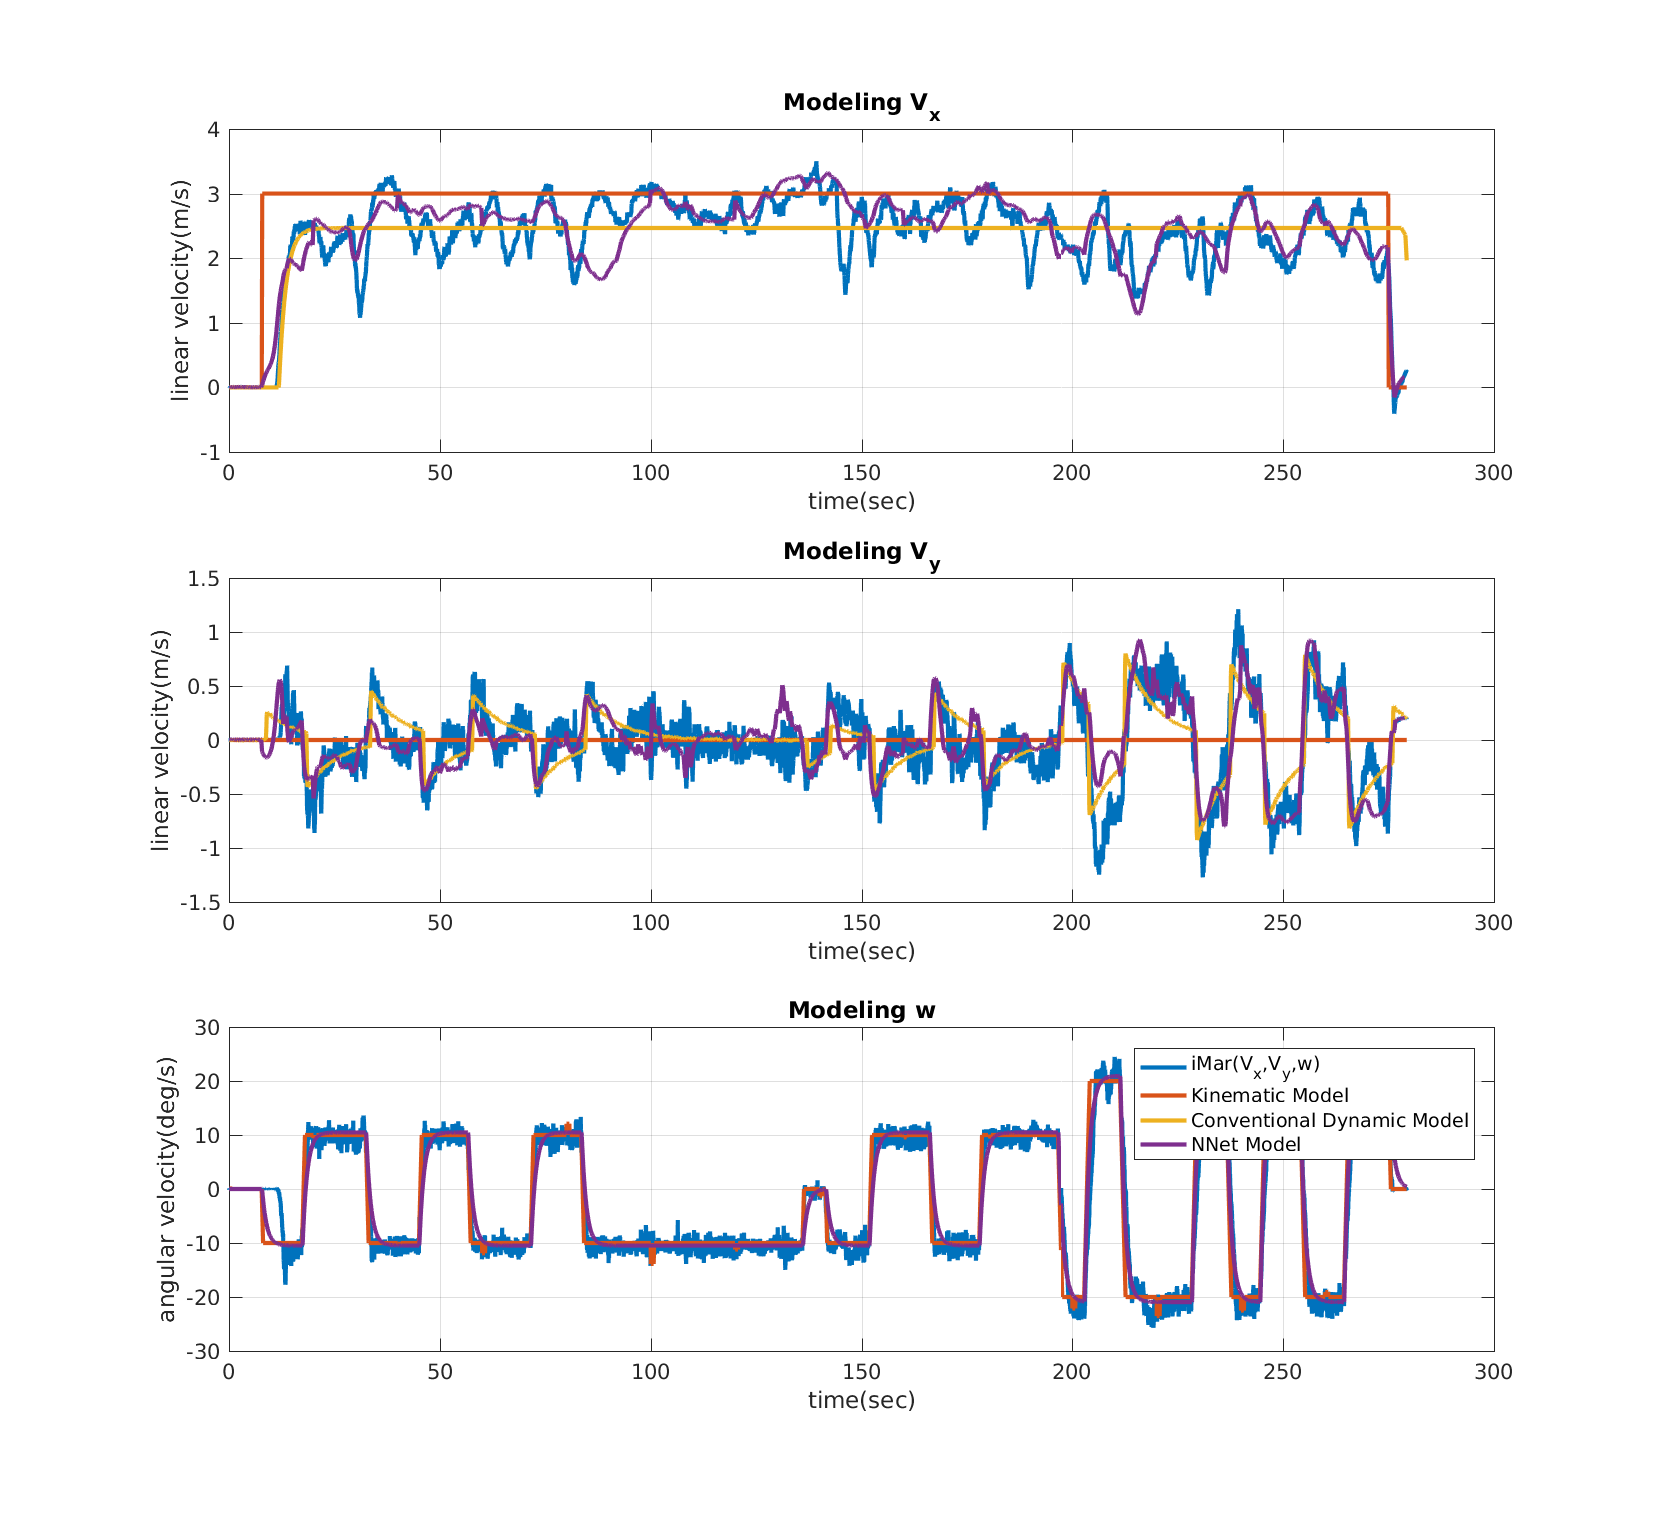
\includegraphics[width=0.8\columnwidth]{./RRTPlanner/fig/simulate_vxvyw}}
           	\caption{Simulated velocity response w.r.t. time steps. Note that the blue line is measured under an accurate GPS/INS sensor with RTK signal. We refer this measurement as our ground true data.}
           	\label{fig:velocity_simulate}
    	\end{center}
\end{figure}
 
\begin{figure}[t]
    	\begin{center}
    	   \centerline{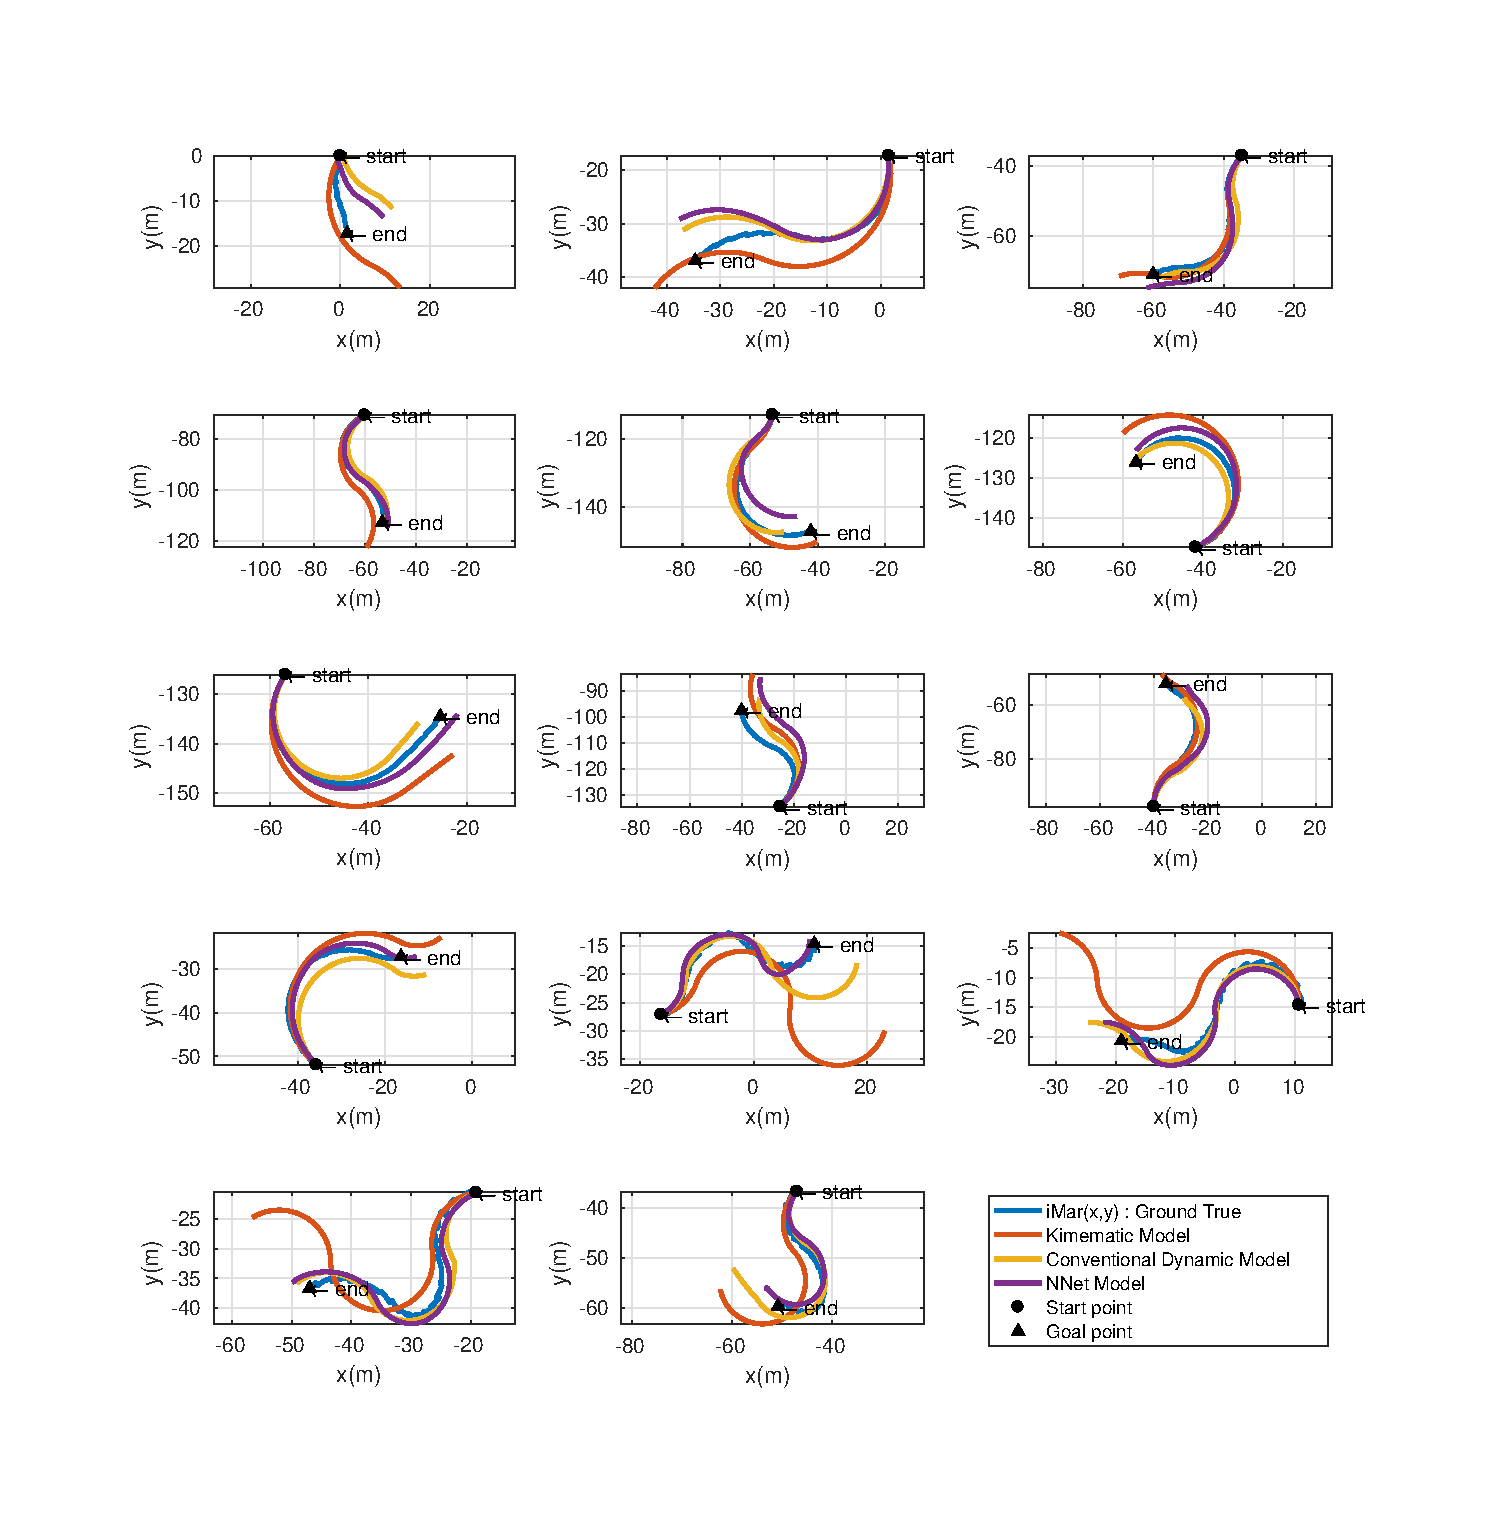
\includegraphics[width=0.8\columnwidth,trim= 0 50 0 160, clip=true]{./RRTPlanner/fig/path_generation_w_nn}}
           	\caption{Comparison between data-driven dynamic model and original kinematic model. Note the time interval in each graph is 20 seconds.}
           	\label{fig:path_generation}
    	\end{center}
\end{figure}
 
%%
Fig. \ref{fig:velocity_simulate} shows the simulated velocity, while Fig. \ref{fig:path_generation} shows the integrated relative position.
The differences between the blue and red line reflect the complexity of vehicle model on the unstructured terrain. 
Integrating directly from control command through time, as shown with the blue line, will give a poor result on state propagation.
Both two proposed models are capable of estimating the lateral velocity, which plays a non-negligible role in off-road cases.
However, the conventional dynamic model is not capable of capturing the nuance variation of the forward velocity. 
The neural net model, on the other hand, gives a better estimation.

% As shown in the blue line in Fig. \ref{fig:velocity_simulate}, the lateral velocity stimulates when the new issued rotational command differs from the previous one, and exponentially decay over time. From this observation, we formulate the lateral velocity response model by using the rotational control to stimulate the peak and fine tuning by a scaling ratio proportional to the forward velocity.
 
 
\subsection{Planner Demo}
 
\begin{figure}[t]
    	\begin{center}
    	 \centerline{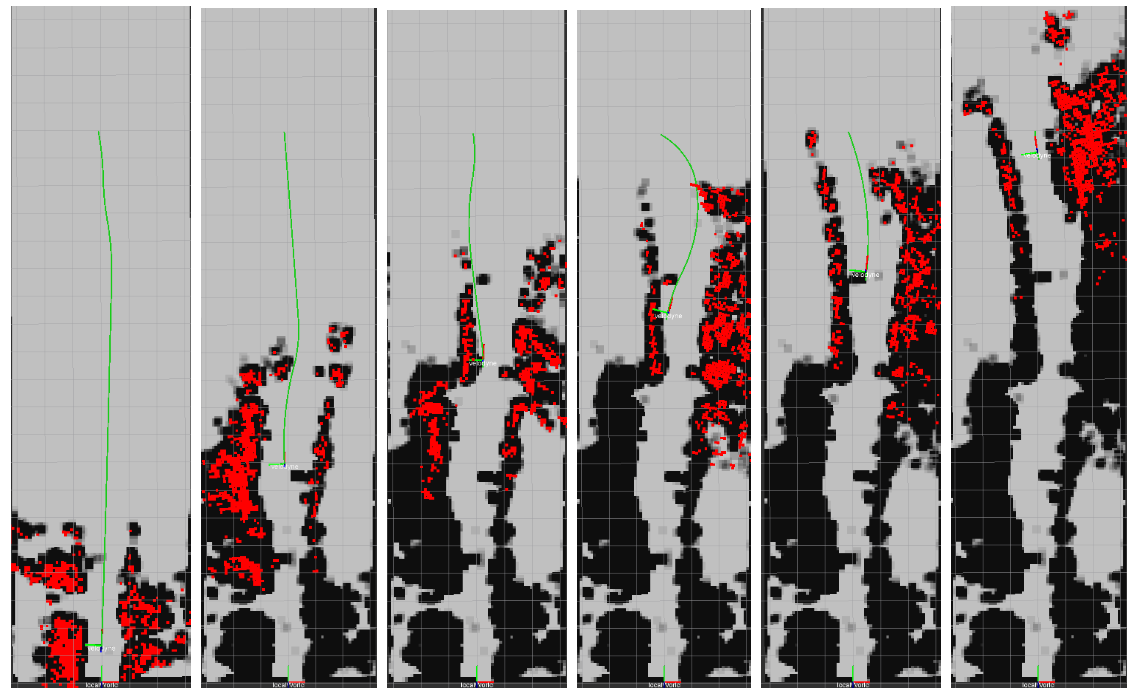
\includegraphics[width=0.8\columnwidth]{./RRTPlanner/fig/demo.png}}
           	\caption{Screenshots of planner visualization output. The green path is the trajectory where each point is encoded with a 6 DoF state, 2 DoF control input, and a control duration. The red points are the filtered point cloud segmented as obstacles.}
           	\label{fig:demo}
    	\end{center}
\end{figure}
 
We test our planner on an off-road test field located near Gascola, Penn Hills, PA.
Our testing scenario is designed as followed: the vehicle should autonomously navigate through a straight turnpike where multiple static obstacles are placed alternatively on both side of the track.
Each static obstacle is 3-meter-length and 1.5-meter height.
The turnpike is a rectangle-shaped field with 10-meter width and 150-meter length.
The fastest way to go through the obstacles without any collisions is to perform S-shape maneuvering.
Since the standard operating speed ranges from $10$ to $40 kph$, we set the baseline testing speed as $20 kph$ with the top speed of $30 kph$.
 
As shown in our demo video
\footnote{On-field testing with path visualization: \url{https://youtu.be/LibnO8_Sjm0}},
the vehicle can successfully avoid all the obstacles at $25 kph$.
However, driving at higher speed ($\sim 30kph$) sometimes makes collision map vulnerable to noises such as dust and sand blown up when the vehicle drives through, which highly affect the path quality outputted by the planner.
The example of planning path generation is visualized in Fig. \ref{fig:demo}.
 
 
\end{document}
